\subsection*{Grafsøk}
\begin{frame}{Søk}
    Om vi har en graf, er det hovedsakelig to måter vi kan søke igjennom grafen: 
    \begin{itemize}
        \item Bredde-Først Søk (BFS)
        \item Dybde-Først Søk (DFS)
    \end{itemize}
    Forskjellen ligger i når hver node blir søkt.
\end{frame}

\begin{frame}[fragile]{BFS: Bredde-Først-Søk}
    Vi holder styr på hvilken 'generasjon' med noder vi jobber med. For hver generasjon ser vi etter alle noder som den generasjonen kan nå, og det er neste generasjon.
    \begin{columns}
        \begin{column}{0.67\textwidth}
            \begin{python}
def bfs(start, graph):
    visited = { u: False for u in graph }
    visited[start] = True
    current_gen = [start]
    next_gen = []
    while len(current_gen) > 0:
        for u in current_gen:
            print(u)
            for v in graph[u]:
                if not visited[v]:
                    next_gen.append(v)
                    visited[v] = True
        current_gen, next_gen = next_gen, []
            \end{python}
        \end{column}
        \begin{column}{0.35\textwidth}
            \begin{figure}
                \centering
                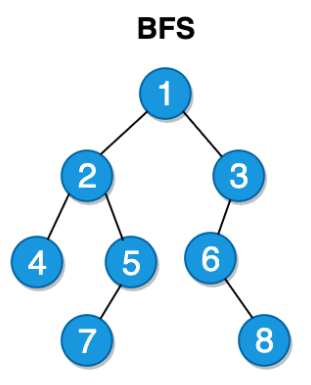
\includegraphics[height=4cm]{images/bfs.png}
            \end{figure}   
        \end{column}
    \end{columns}
\end{frame}

\begin{frame}[fragile]{DFS: Dybde-Først-Søk}
    Her går vi heller i dybden først. Hver gang vi oppdager en ny node søker vi den umiddelbart før vi går tilbake igjen.
    \begin{columns}
        \begin{column}{0.5\textwidth}
            \begin{python}
def dfs(start, graph, visited):
    print(start)
    visited[start] = True
    for v in graph[start]:
        if not visited[v]:
            dfs(v, graph, visited)
            \end{python}
        \end{column}
        \begin{column}{0.45\textwidth}
            \begin{figure}
                \centering
                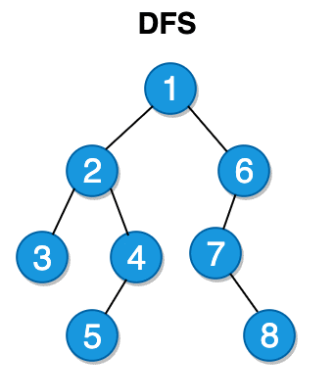
\includegraphics[height=4cm]{images/dfs.png}
            \end{figure}   
        \end{column}
    \end{columns}
\end{frame}